\section{La Détection de Relations Sémantiques}

Etant donné que le réseau encode de nombreuses relations sémantiques 
différentes qui sont a priori identifiables par les poids attribués, il devrait 
être possible dans une certaine mesure d'identifier ces relations ou de mettre 
certaines relations en avant. Nous avons de nombreux paramètres qui peuvent être 
modifiés pour changer les valeurs données à certaines relations et l'objectif 
est de trouver les paramètres qui optimise certaines relations. La relation la 
plus évident à vouloir chercher est celle de la synonymie, qui est une relation 
entre deux mots qui ont le même sens (approximativement). Comme suggéré au 
début, cette relation est en réalité difficilement définissable, surtout par 
rapport aux nuances de sens que peuvent prendre des mots. La relation entre 
\lq{content}\rq{} et \lq{joyeux}\rq est certes évidente mais le linguiste motivé 
peut toujours justifié une différence de sens entre les deux, quoique légère.

Au lieu de rentrer dans les détails du débat de la synonymie, nous jugeons et 
évaluons nos relations de synonymie trouvées par rapport aux ressources 
externes, qui encode des relations de synonymie. Il est fort possible que ces 
ressources ne contiennent pas toutes les relations de synonymie existantes, mais 
ce sont des avis externes et établis qui fournissent un premier moyen de juger 
si le réseau sémantique établit bien des relations de synonymie.

\subsection{Détection de synonymes}

L'application est très simple et se base sur le parcours en largeur décrit dans 
la section [REF]. Elle fait un appel à ce parcours pour chercher les k plus 
proches voisins d'un mot donné. Ce mot peut être associé à une catégorie 
syntaxique ou pas. La catégorie syntaxique du mot cible peut également être 
spécifiée, permettant de chercher éventuellement des relations autre que la 
synonymie (si les catégories source et cible sont différentes).

La liste des voisins (un maximum de k) est renvoyé, ainsi que le chemin 
emprunté pour y arriver et la distance entre le mot source et le mot cible.

\subsubsection{L'Interface}

L'interface est réalisée en utilisant les bibliothèques Tkinter [REF] et PMW 
[REF] sous python.

\begin{center}
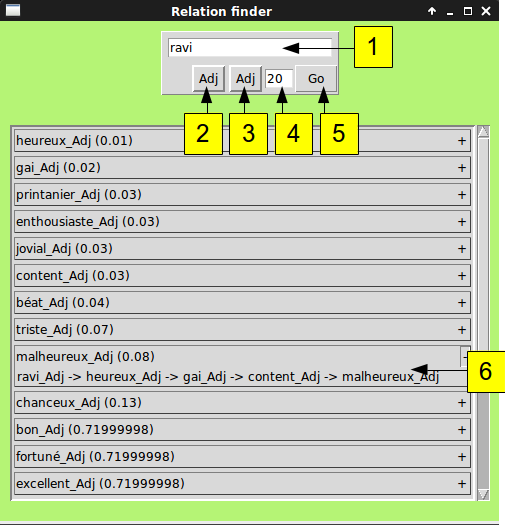
\includegraphics[width=13cm]{relationfinderinterface.png}
\end{center}

\begin{enumerate}
    \item{L'utilisateur peut écrire un mot à rechercher ici}
    \item{Le choix de catégorie syntaxique du mot source parmi une liste 
    d'options. L'option ``*" par défaut signifie que le mot recherché peut être 
    de n'importe quelle catégorie}
    \item{Le choix de catégorie des mots cibles. La liste d'options est la même 
    que pour la catégorie source et peut ne pas correspondre à la catégorie 
    source.}
    \item{Le nombre de voisins à renvoyer. Dans le cas où un mot est relié à 
    moins de voisins que demandés, le maximum de voisins sera renvoyé.}
    \item{Pour lancer une recherche du réseau}
    \item{Les voisins sont affichés avec leur distance entre parenthèses. Le 
    chemin est affiché en cliquant sur le signe \lq{+}\rq{}}   

\end{enumerate}

\subsubsection{Optimisation}

L'objectif principal est de maximiser le nombre de mots trouvés qui 
correspondent à la relation de synonymie. Le fait que les paramètres différents 
pour la création et le parcours de la matrice (détaillée en section [REF]) 
soient des valeurs numériques permet d'envisager une optimisation automatique de 
ces valeurs.

Il s'agit, à partir d'un corpus d'entraînement et un vecteur de paramètres de 
regénérer la matrice et évaluer les résultats contre les ressources [REF]XXX 
pour trouver les valeurs qui donnent le meilleur score.

Le vecteur de paramètres comprend les valeurs associées aux types de relations 
(ex: pos2entry, sense2deftext, ...) et les autres paramètres détaillés dans la 
section [REF]. La récupération de ce vecteur est incorporé dans le programme 
pour la création de la matrice, qui contient aussi des méthodes pour changer les 
valeurs de ces paramètres et pour les réécrire dans les fichiers de 
configuration.

PARTIE SUR LA FONCTION D'EVALUATION... (je ne veux pas le refaire pour 
l'instant - Caro - tu peux mettre ta partie ici ?)

L'évaluation selon le corpus se fait en utilisant un métrique défini par 
nous-mêmes pour juger de la qualité des résultats renvoyés par la recherche. 
Etant donné que les premiers mots dans la liste sont censés être les plus 
proches du mot cible, il est important d'incorporer une notion de l'emplacement 
d'un synonyme trouvé dans la liste de résultats.

DESCRIPTION DU METRIQUE

La bibliothèque Scipy [REF] fournit une méthode \lq{minimize}\rq{} qui sert à 
minimiser la valeur retourner d'une fonction à partir d'un vecteur de 
paramètres.

FINIR



\subsection{Evaluation}

L'évaluation de RelationFinder s'est faite en deux temps. D'abord grâce à des 
données récupérées dans le corpus wolf puis grâce à des données récuppérées sur 
le site de Crisco.

Pour faire cette évaluation nous regardons le mot à traiter puis nous cherchons 
ses k plus proches voisins (dans notre évaluation k = 19). Si l'un des 
synonymes du corpus est dans les k plus proches voisins. On donne un score à ce 
synonyme.

Le score est calculé par rapport à la place du synonymes dans les voisins. Si 
le synonyme est 3ème sur le 19 voiin il aura un score de 19 - 3 => 16. Si il 
est 17ème il aura un score de 19 - 17 => 2.

Dans le même temps nous calculons le score maximum qu'il est possible d'avoir. 
C'est-à-dire k - len(syns). Si dans le corpus nous avons 5 synonymes alors le 
score maximum sera 19 + 18 + 17 + 16 + 15 => 85.

Pour calculer l'exactitude de notre RelationFinder nous finissons donc par 
diviser le score de tous nos synonymes trouvés par le score maximum total.

Il faut donc bien noter que k ne doit pas être inférieur au nombre maximal de 
Synonymes sinon les résultats peuvent tomber en négatif \dots

\subsubsection{wolf}

Le corpus wolf a été réalisé à partir du Princeton WordNet et diverses autres 
ressources multilingues. Il a été évaluer par rapport au WordNet français.

Dans le corpus wolf nous n'avons récupérés que les données ayant été validées 
manuellement. Pour être sûrs de ne pas avoir de bruit dû à quelques ambiguïtés.

Notre extrait de wolf contient 120 mots ainsi que leurs synonymes dans le 
corpus. Chaque mot possède entre 1 et 8 synonymes.

\subsubsection{Crisco}

Le corpus crisco est un petit corpus que nous avons réalisé nous-même pour voir 
si la source du corpus pouvait modifier grandement ou non l'exactitude obtenue 
lors de l'évaluation. Nous avons créé ce corpus en entrant les différents mots 
dans la base de données crisco disponible en ligne.

Notre corpus est composé de 78 mots ayant chacun entre 1 et 10 synonymes.
